% Load preamble
\documentclass[../main.tex]{subfiles}
\usepackage{rotating}

\begin{document}
	
\subsection{Úvodný príklad}
Uvažujme nelineárny systém, opísaný stavovými rovnicami \ref{eqn:Rovnica1}, ktorého bloková schéma je zobrazená na obrázku \ref{fig:BlokovaSchemaPr1}. 

\begin{equation}
	\begin{gathered}
	\dot{x_1}  = x_1^2 + x_2 - x_1 \\
	\dot{x_2} = u - x_1 - x_2 \\
	\end{gathered}
	\label{eqn:Rovnica1}
\end{equation}
	
\begin{figure}[H]
	\begin{center}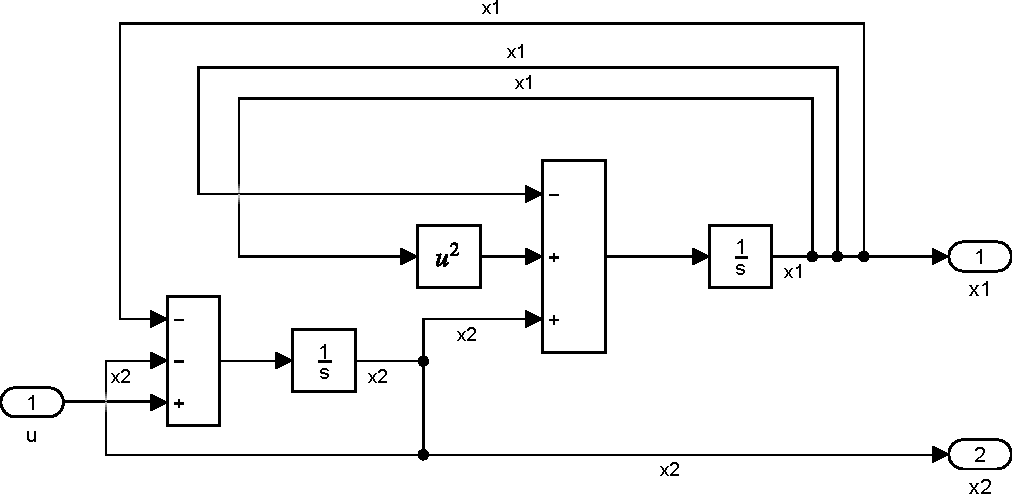
\includegraphics[scale=0.8]{Rovnica1.pdf}\end{center}
	\caption{Bloková schéma systému \ref{eqn:Rovnica1}}
	\label{fig:BlokovaSchemaPr1}
\end{figure}
	
\subsection{Metóda vstupno-stavovej spätnoväzobnej linearizácie}

Na riadenie nelineárneho systému (rovnica \ref{eqn:Rovnica1}), použijeme metódu vstupno-stavovej spätnoväzobnej linearizácie (obrázok \ref{fig:MetodaVS}), tak aby sme dosiahli požadovanú hodnotu $r$.

\begin{figure}[H]
	\begin{center}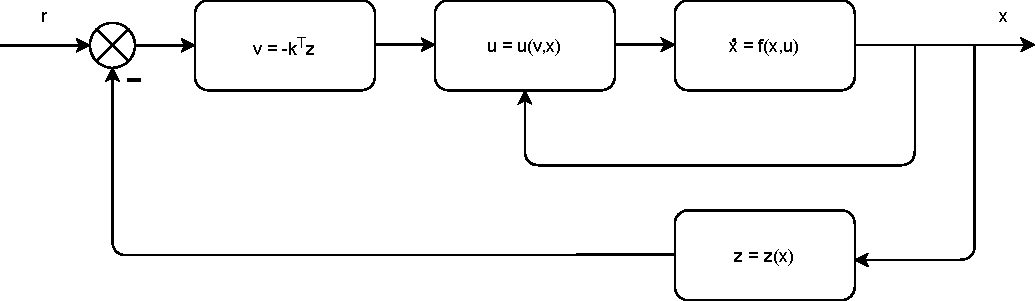
\includegraphics[scale=0.8]{MVSlin.pdf}\end{center}
	\caption{Metóda vstupno-stavovej spätnoväzobnej linearizácie}
	\label{fig:MetodaVS}
\end{figure}

Postup pri metóde vstupno-stavovej spätnoväzobnej linearizácie je nasledovný.\\\\
Najskôr si určíme transformačné vzťahy, tzn. určíme vektor $r$.
\begin{equation}
	\begin{gathered}
		z_1  = x_1 \\
		z_2 = x_1^2 + x_2 \\
	\end{gathered}
	\label{eqn:TransformacneVztahy}
\end{equation}
Následne transformujeme zadaný nelineárný systém (rovnica \ref{eqn:Rovnica1}), pomocou nájdených transformačných vzťahov (rovnica \ref{eqn:TransformacneVztahy}).
\begin{equation}
	\begin{split}
	\dot{z_1}  & = \dot{x_1} = z_2 - z_1 \\
	\dot{z_2} & = 2x_1\dot{x_1} + \dot{x_2} \\
	 & = 2x_1(x_1^2 + x_2 - x_1) + u - x_1 - x_2 \\
	 & = 2z_1(z_2 - z_1) + u - z_1 - z_2 + z_1^2\\
	 & = u - z_1^2 + 2z_1z_2 - z_1 - z_2 \\
	\end{split}
	\label{eqn:TransformovanySystem}
\end{equation}

Aby sme dosiali lineárny transformovaný systéme zavedieme novú premennú $v$.

\begin{equation}
	\begin{split}
	 v = u - z_1^2 + 2z_1z_2 - z_1 - z_2 \\
	\end{split}
	\label{eqn:SubsV}
\end{equation}

Z trasformovanej sústavy získame vzťah pre nelineárne riadenie, akčný zásah $u$.

\begin{equation}
	\begin{gathered}
		u = v + z_1^2 - 2z_1z_2 + z_1 + z_2\\
	\end{gathered}
	\label{eqn:Noveu}
\end{equation}

Zavedením novej premennej sme získali nový transformovaný lineárny systém.

\begin{equation}
	\begin{split}
	\dot{z_1}  & = z_2 - z_1 \\
	 \dot{z_2} & = v \\
	\end{split}
	\label{eqn:TransformovanySystem}
\end{equation}

Po získaní lineárneho systému môžeme zaviesť lineárny stavový regulátor (rovnica \ref{eqn:LinReg}).
\begin{equation}
	\begin{split}
		v = k_1z_1 + k_2z_2 \\
	\end{split}
	\label{eqn:LinReg}
\end{equation}

Lineárny systém s regulátorom bude vyzerať nasledovne: rovnica \ref{eqn:TransformovanySystemSRegulatorom}. 
\begin{equation}
	\begin{split}
	\dot{z_1}  & = z_2 - z_1 \\
	 \dot{z_2} & = k_1z_1 + k_2z_2 \\
	\end{split}
	\label{eqn:TransformovanySystemSRegulatorom}
\end{equation}

Na vypočítanie parametrov regulátora a nastavenie dynamiky systému potrebujeme odvodiť charakteristickú rovnicu systému.
Na získanie charakteristickej rovnice potrebujeme získať maticu $A$.
\begin{equation}
\begin{split} 
 A  & = \begin{bmatrix} \frac{\partial \dot{z_1}}{\partial z_1}& \frac{\partial \dot{z_1}}{\partial z_2}\\ \frac{\partial \dot{z_2}}{\partial z_1}&\frac{\partial \dot{z_2}}{\partial z_2} \end{bmatrix}_{|_{z_1 = z_2 = 0}} \\
 & = \begin{bmatrix} -1 & 1\\ k_1 & k_2 \end{bmatrix} \
 \end{split}
 \label{eqn:A}
\end{equation}
Charakteristickú rovnicu získame z rovnice \ref{eqn:CHR}.
\begin{equation}
\begin{split} 
 |\lambda I - A| & = 0\\
|\lambda I - A| & = \begin{bmatrix} \lambda +1 & -1\\ -k_1 & \lambda -k_2 \end{bmatrix} \\
|\lambda I - A| & = (\lambda + 1)(\lambda - k_2) - k_1\\
\lambda^2 - \lambda(k_2+1) - k_1 &= 0\\ 
\end{split}
\label{eqn:CHR}
\end{equation}

Vieme, že korene charakteristickej rovnice musia ležať v zápornej polrovine. Preto si zvolíme korene $\lambda_1 = -1$,$\lambda_2 = -2$, pomocou ktorých získame parametre $k_1,k_2$ (rovnica \ref{eqn:Korene}).

\begin{equation}
\begin{split} 
\lambda^2 - \lambda(k_2+1) - k_1 & = (\lambda + 1)(\lambda + 2)\\ 
\lambda^2 - \lambda(k_2+1) - k_1 & = \lambda^2 + 3\lambda + 2\\ 
k_1 &= -2\\
k_2 &= -4\\
\end{split}
\label{eqn:Korene}
\end{equation}

Výsledky overíme simulačne pomocou schémy na obrázku \ref{fig:PrikladsRiadenim}.

\newpage
	

\begin{figure}[H]
	\begin{center}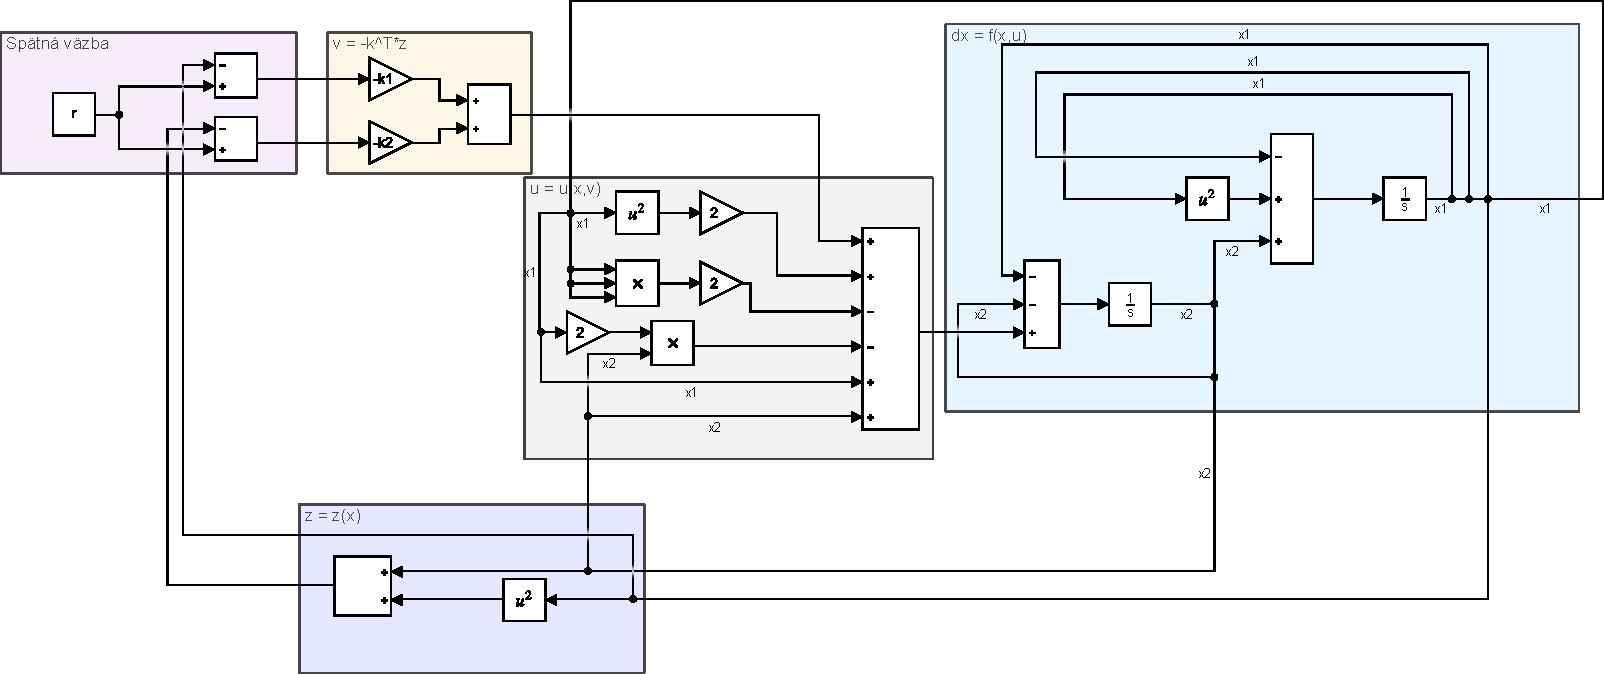
\includegraphics[scale=0.8,angle=90]{Rovnica1MVS.pdf}\end{center}
	\caption{Bloková schéma systému}
	\label{fig:PrikladsRiadenim}
\end{figure}


\newpage
\subsection{Záver}

Z výsledkov simulácie, ktoré su zobrazené na obrázkoch \ref{fig:Vysledok1}, \ref{fig:Vysledok2}, môžeme vidieť, že s pomocou navrhnutého riadenia pre nelinárny systém sme dokázali dosiahnúť požadovanú hodnotu $r$.

\begin{figure}[H]
	\begin{center}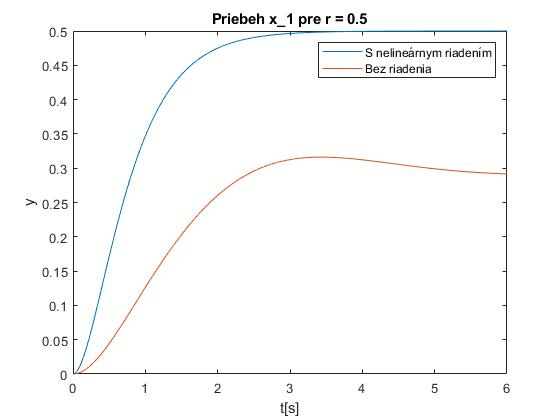
\includegraphics[scale=0.6]{r05.jpg}\end{center}
	\caption{Bloková schéma systému}
	\label{fig:Vysledok1}
\end{figure}
\begin{figure}[H]
	\begin{center}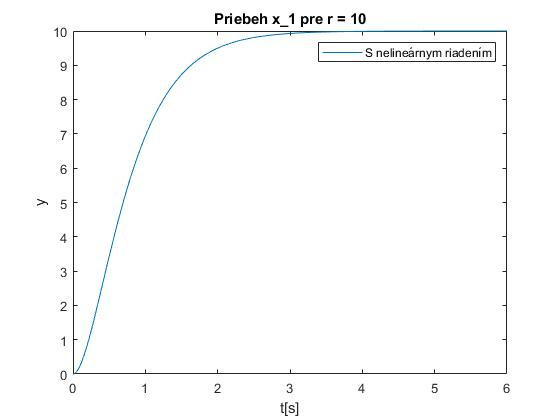
\includegraphics[scale=0.6]{r10.jpg}\end{center}
	\caption{Bloková schéma systému}
	\label{fig:Vysledok2}
\end{figure}
	
\end{document}
